\section{Computational Evaluation}
\label{sec:results}

The computational evaluation begins with a numerical validation
against PySCF and then turns to model-capability tests. The validation
module checks that GradTDDFT reproduces conventional TDA and full
TDDFT excitation energies, oscillator strengths, and response
matrices before neural parameters are introduced. The capability
tests then ask whether differentiable neural exchange-correlation
functionals can learn ground-state surfaces, excited-state response,
and molecular ground-state and vertical-excitation targets
within a shared SCF--TDDFT implementation. These model tests are
divided into two blocks: bond-dissociation curves covering
ground-state surfaces and first excited-state response, and
separate ground-state and excited-state training on a 50-molecule QM9
subset.

Across all experiments, the recorded computational state includes the
geometry source, charge and spin multiplicity, basis set, quadrature
grid, SCF convergence criteria, TDDFT solver, excited-state treatment,
backend/device, training seed, and reference method. These records are
part of the benchmark definition because small changes in grids,
spin treatment, or SCF convergence can otherwise obscure whether an
observed error comes from the learned functional or from the numerical
setup.

% ======================================================================
\subsection{Numerical Validation against PySCF}
\label{sec:eval-pyscf}

The first evaluation module isolates the TDDFT response construction
before any neural functional parameters are trained. In the
conventional-functional limit, GradTDDFT evaluates the
exchange-correlation energy density as a differentiable function of
the density descriptors and obtains both the potential and the local
response tensor by automatic differentiation,
\begin{equation}
  E_{\rm xc}
  \longrightarrow
  v_{\rm xc}
  =
  \frac{\delta E_{\rm xc}}{\delta \rho}
  \longrightarrow
  f_{\rm xc}
  =
  \frac{\delta v_{\rm xc}}{\delta \rho}.
\end{equation}
The resulting tensor is contracted with quadrature weights and AO
basis values, transformed to the occupied--virtual orbital basis, and
inserted into the TDA or Casida response matrices. Matched PySCF
calculations provide independent references for the same geometry,
functional, basis, grid, SCF solution, and response equations.

The validation matrix contains H$_2$O, CO, N$_2$, C$_2$H$_4$,
formaldehyde, benzene, and OH with PBE, B3LYP, and PBE0 in def2-SVP
and aug-cc-pVDZ basis sets. Restricted KS references are used for the
closed-shell molecules, while unrestricted KS references are used for
OH. For each matched setup, TDA and full TDDFT are evaluated for the
first five singlet and triplet states where the reference calculation
is defined.

For the PBE/def2-SVP subset reported here, all 26 calculations
completed successfully, giving 130 per-state records. The direct
GradTDDFT--PySCF comparison contains 12 restricted-singlet tasks,
corresponding to 60 excitation states across TDA and full TDDFT. The
excitation-energy mean absolute differences relative to PySCF range
from \(5.86\times 10^{-14}\) to \(2.87\times 10^{-10}\) eV, with
maximum absolute state errors below \(5.47\times 10^{-10}\) eV.
Oscillator-strength mean absolute differences range from
\(1.86\times 10^{-22}\) to \(1.29\times 10^{-7}\). For response
matrices small enough to store explicitly in this audit, the RMS
differences in the assembled \(A\) and \(B\) matrices are
\(5.65\times 10^{-15}\) to \(8.26\times 10^{-15}\).

\begin{table}[t]
\centering
\caption{B3LYP/def2-SVP S$_1$ excitation energies and oscillator
strengths from matched PySCF and GradTDDFT calculations. Each entry
reports \(\Omega_1\) in eV followed by \(f_1\).}
\label{tab:b3lyp-s1-excitation-oscillator}
\begin{tabular}{llcc}
\toprule
Molecule & Solver & PySCF & GradTDDFT \\
\midrule
H$_2$O & TDA & 7.6 / \(1.8\times 10^{-2}\) & 7.6 / \(1.8\times 10^{-2}\) \\
H$_2$O & TDDFT & 7.6 / \(1.8\times 10^{-2}\) & 7.6 / \(1.8\times 10^{-2}\) \\
CO & TDA & 8.7 / \(1.1\times 10^{-1}\) & 8.7 / \(1.1\times 10^{-1}\) \\
CO & TDDFT & 8.5 / \(8.2\times 10^{-2}\) & 8.5 / \(8.2\times 10^{-2}\) \\
N$_2$ & TDA & 9.5 / \(4.5\times 10^{-31}\) & 9.5 / \(3.4\times 10^{-31}\) \\
N$_2$ & TDDFT & 9.4 / \(4.7\times 10^{-18}\) & 9.4 / \(7.2\times 10^{-25}\) \\
C$_2$H$_4$ & TDA & 8.3 / \(5.4\times 10^{-29}\) & 8.3 / \(6.0\times 10^{-29}\) \\
C$_2$H$_4$ & TDDFT & 8.1 / \(3.7\times 10^{-1}\) & 8.1 / \(3.7\times 10^{-1}\) \\
CH$_2$O & TDA & 4.0 / \(1.9\times 10^{-29}\) & 4.0 / \(1.8\times 10^{-29}\) \\
CH$_2$O & TDDFT & 4.0 / \(2.2\times 10^{-25}\) & 4.0 / \(5.4\times 10^{-29}\) \\
C$_6$H$_6$ & TDA & 5.5 / \(3.7\times 10^{-9}\) & 5.5 / \(3.7\times 10^{-9}\) \\
C$_6$H$_6$ & TDDFT & 5.5 / \(4.9\times 10^{-9}\) & 5.5 / \(4.9\times 10^{-9}\) \\
\bottomrule
\end{tabular}
\end{table}

This validation establishes the numerical equivalence of the
differentiable TDDFT path and matched PySCF calculations for
traditional functionals. The following sections therefore evaluate
model behavior rather than basic response-matrix assembly.

% ======================================================================
\subsection{\texorpdfstring{Ground- and Excited-State Dissociation Curves}{Ground- and Excited-State Dissociation Curves}}
\label{sec:eval-dissociation}
\label{sec:eval-ground-dissociation}
\label{sec:eval-excited-dissociation}

The first model-capability benchmark evaluates one-dimensional bond
dissociation curves for H$_2$, H$_2^+$, and N$_2$, with first
excited-state scans for H$_2$ and N$_2$. The H$_2$/H$_2^+$
pair follows the Kohn--Sham regularizer benchmark of Li
\emph{et al.}: H$_2$ is a compact bond-breaking and
strong-correlation test, whereas H$_2^+$ isolates one-electron
self-interaction and open-shell SCF stability.\cite{Li2021KohnShamRegularizer}
N$_2$ extends this setting to a stretched multiple bond; recent
high-level spectroscopic calculations treat molecular nitrogen as a
dense multi-state problem, reporting potential-energy curves and
transition dipole moments for the 51 lowest electronic states over
1.35--10 bohr and multiple N + N dissociation
limits.\cite{Hammami2026N2PEC} The three systems therefore separate
self-interaction, two-electron bond breaking, and stretched
triple-bond near-degeneracy within a small set of scans.
The ground-state curves are labeled by the corresponding
diatomic spectroscopic terms, \(X\,{}^1\Sigma_g^+\) for H$_2$
and N$_2$ and \(X\,{}^2\Sigma_g^+\) for H$_2^+\). The excited-state
curves are labeled as H$_2$ \(B\,{}^1\Sigma_u^+\) and N$_2$
\(A\,{}^1\Pi_g\); the latter follows the large-CAS state assignment
used in the N$_2$ reference data.\cite{Hammami2026N2PEC}

The results are organized around the physically meaningful channel for
each system. For the one-electron H$_2^+$ ion, the MP2/PT2 doubles
space is empty, so a PT2 correction is identically zero and does not
provide a useful functional test. H$_2^+$ is therefore used to compare
implicit-SCF training with fixed-density training. For H$_2$ and N$_2$,
the implicit-SCF protocol is used throughout, and the PT2/no-PT2
comparison tests how strongly the second-order channel improves the
learned functional along bond dissociation. The H$_2$ and N$_2$ first
excited-state dissociation curves apply the same PT2-channel test to
the TDDFT response calculation. The curve-plus-error layout, training
markers, and chemical accuracy band are used as direct diagnostics,
with convergence success, cycle count, and failure rate recorded at
every geometry.

\begin{figure}[!htbp]
\centering
\begin{minipage}{0.49\linewidth}
  \centering
  \textbf{(a) Implicit SCF}\\[-0.3em]
  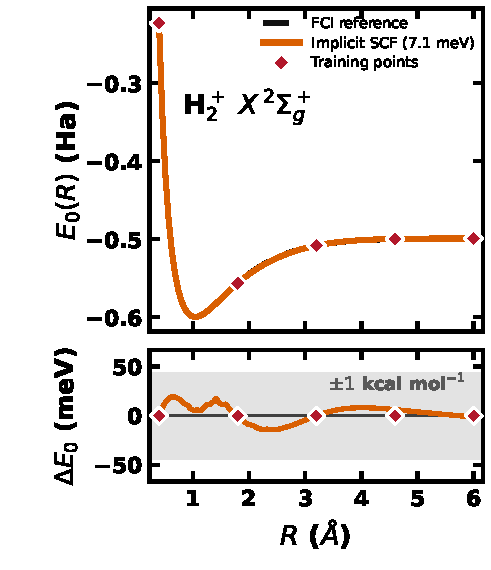
\includegraphics[width=\linewidth]{figures/h2plus_ground_hfx_implicit_scf_dissociation_paper_style.pdf}
\end{minipage}
\hfill
\begin{minipage}{0.49\linewidth}
  \centering
  \textbf{(b) Fixed density}\\[-0.3em]
  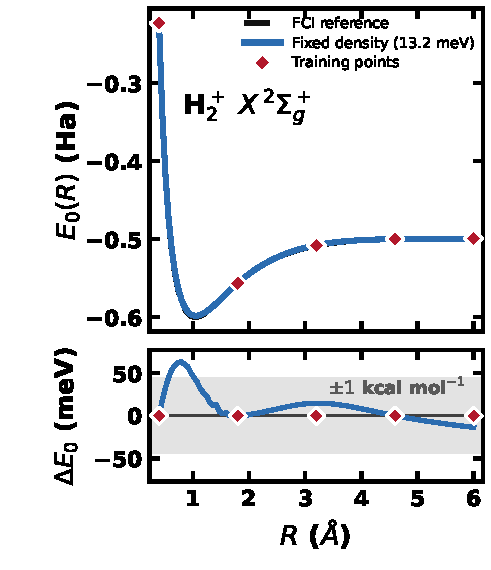
\includegraphics[width=\linewidth]{figures/h2plus_ground_hfx_fixed_density_dissociation_paper_style.pdf}
\end{minipage}
\caption{H$_2^+$ \(X\,{}^2\Sigma_g^+\) ground-state dissociation
curves for the HFX-channel neural functional under implicit-SCF and
fixed-density training. In
each panel, the upper subpanel compares the learned curve with the
one-electron FCI reference values, while the lower subpanel shows the
signed error
\(\Delta E_0=E_{0,\rm model}-E_{0,\rm ref}\). Red diamonds denote the
five training geometries, and the gray band marks
\(\pm 1\) kcal mol\(^{-1}\). The implicit-SCF model gives a dense-curve
mean absolute error of 7.1 meV and a maximum absolute error of
19.2 meV. Fixed-density training gives corresponding errors of
13.2 meV and 63.2 meV.}
\label{fig:h2plus-ground-hfx-dissociation}
\end{figure}

\begin{figure}[!htbp]
\centering
\begin{minipage}{0.485\linewidth}
  \centering
  \textbf{(a) H$_2$, HFX+PT2}\\[-0.3em]
  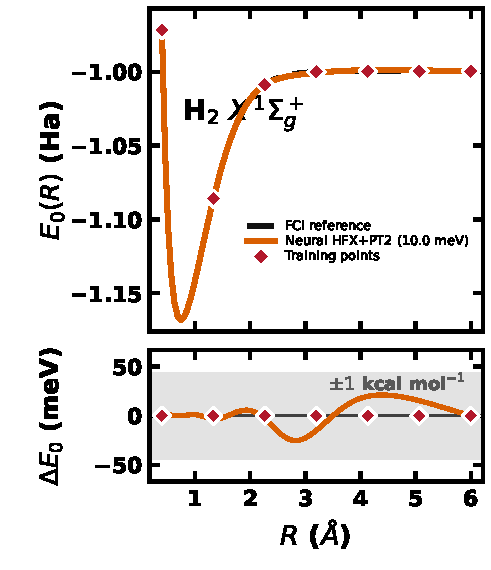
\includegraphics[width=0.88\linewidth]{figures/h2_ground_hfx_pt2_dissociation_paper_style.pdf}
\end{minipage}
\hfill
\begin{minipage}{0.485\linewidth}
  \centering
  \textbf{(b) H$_2$, HFX/no-PT2}\\[-0.3em]
  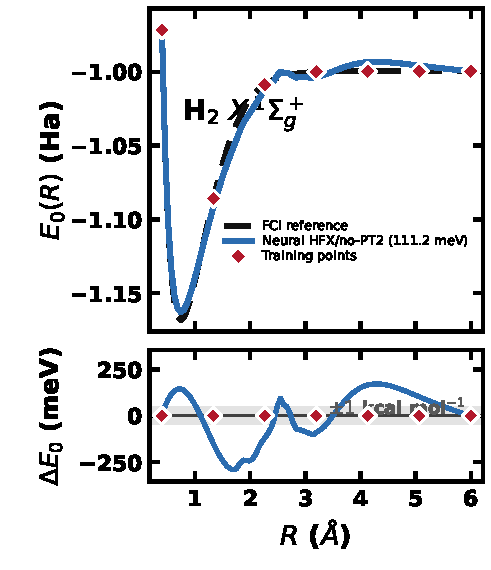
\includegraphics[width=0.88\linewidth]{figures/h2_ground_hfx_nopt2_dissociation_paper_style.pdf}
\end{minipage}\\[-0.2em]
\begin{minipage}{0.485\linewidth}
  \centering
  \textbf{(c) N$_2$, HFX+PT2}\\[-0.3em]
  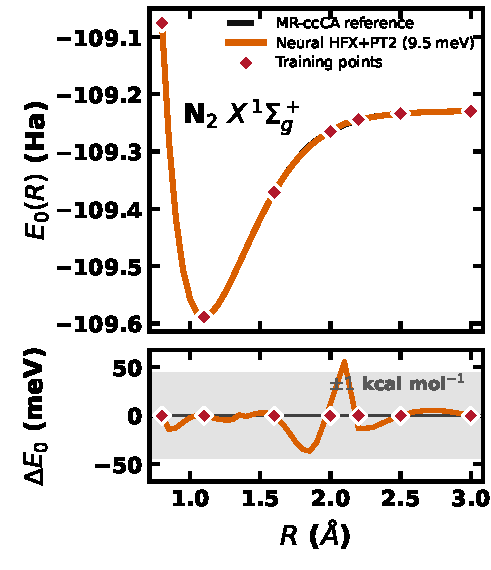
\includegraphics[width=0.88\linewidth]{figures/n2_ground_hfx_pt2_dissociation_paper_style.pdf}
\end{minipage}
\hfill
\begin{minipage}{0.485\linewidth}
  \centering
  \textbf{(d) N$_2$, HFX/no-PT2}\\[-0.3em]
  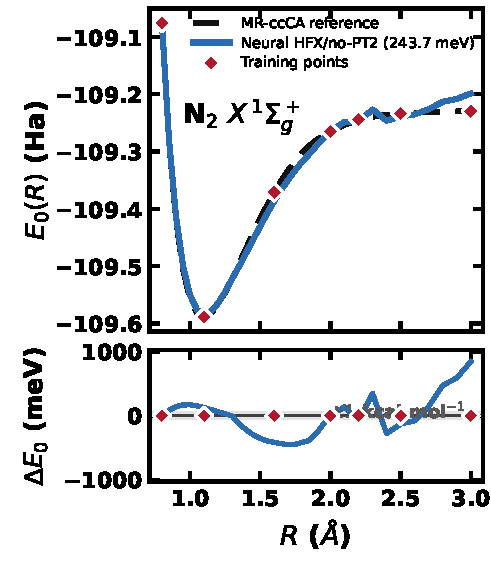
\includegraphics[width=0.88\linewidth]{figures/n2_ground_hfx_nopt2_dissociation_paper_style.pdf}
\end{minipage}
\caption{H$_2$ and N$_2$ \(X\,{}^1\Sigma_g^+\) ground-state
dissociation curves for neural functionals trained with and without
the PT2 channel. In each panel,
the upper subpanel compares the learned curve with the reference
values, while the lower subpanel shows the signed error
\(\Delta E_0=E_{0,\rm model}-E_{0,\rm ref}\). Red diamonds denote the
seven training geometries, and the gray band marks
\(\pm 1\) kcal mol\(^{-1}\). For H$_2$, the HFX+PT2 model gives a
dense-curve mean absolute error of 10.0 meV and a maximum absolute
error of 25.4 meV, while removing the PT2 channel increases the
corresponding errors to 111.2 meV and 292.1 meV. For N$_2$, the
HFX+PT2 model gives corresponding errors of 9.5 meV and 55.7 meV,
whereas the HFX/no-PT2 model gives 243.7 meV and 844.0 meV.}
\label{fig:h2-n2-ground-hfx-pt2-nopt2-dissociation}
\label{fig:h2-ground-hfx-pt2-nopt2-dissociation}
\label{fig:n2-ground-hfx-pt2-nopt2-dissociation}
\end{figure}

\begin{figure}[!htbp]
\centering

\includegraphics[width=0.86\linewidth]{figures/h2_s1_tda_e1_total_pt2_nopt2_dissociation_paper_style.pdf}
\caption{H$_2$ \(B\,{}^1\Sigma_u^+\) excited-state dissociation curve
for neural TDA calculations with and without the PT2 channel. The
plotted quantity is the total excited-state energy
\(E_1(R)=E_0(R)+\Omega_1(R)\). In each panel, the upper subpanel
compares the learned curve with the FCI reference values, while the
lower subpanel shows the signed error
\(\Delta E_1=E_{1,\rm model}-E_{1,\rm ref}\). Red diamonds denote the
training geometries, and the gray band marks
\(\pm 1\) kcal mol\(^{-1}\). The PT2-channel model gives a dense-curve
mean absolute error of 35.9 meV and a maximum absolute error of
208.0 meV, whereas the updated no-PT2 model gives corresponding
errors of 70.1 meV and 199.3 meV.}
\label{fig:h2-s1-tda-e1-total-pt2-nopt2-dissociation}
\end{figure}

\begin{figure}[!htbp]
\centering

\includegraphics[width=0.86\linewidth]{figures/n2_s1_tda_e1_total_pt2_nopt2_dissociation_paper_style.pdf}
\caption{N$_2$ \(A\,{}^1\Pi_g\) excited-state dissociation curves for
neural TDA calculations with and without the PT2 channel. The plotted
quantity is the total excited-state energy
\(E_1(R)=E_0(R)+\Omega_1(R)\), using the Hammami
\emph{et al.} large-CAS curve as the reference.\cite{Hammami2026N2PEC}
In each panel, the upper subpanel compares the learned
curve with the reference values, while the lower subpanel shows the
signed error
\(\Delta E_1=E_{1,\rm model}-E_{1,\rm ref}\). Red diamonds denote the
training geometries, and the gray band marks
\(\pm 1\) kcal mol\(^{-1}\). The PT2-channel model gives a dense-curve
mean absolute error of 0.161 eV and a maximum absolute error of
0.477 eV, while removing the PT2 channel increases the corresponding
errors to 0.871 eV and 2.905 eV.}
\label{fig:n2-s1-tda-e1-total-pt2-nopt2-dissociation}
\end{figure}

\subsection{Semi-local Channel Composition Tests}
\label{sec:semilocal-channel-composition}

The dissociation benchmarks above vary the implicit-SCF treatment and
the second-order PT2 channel. A complementary training test asks a
narrower question: under a fixed \texttt{noPT2}+HFX implicit-SCF
protocol, how strongly does the semi-local channel basis affect the
N$_2$ ground-state and first-excited-state dissociation curves? In
this comparison, the MP2/PT2 channel is disabled, the local
exact-exchange descriptor \(h_g\) remains active through
\(c_x^\theta(\mathbf{z}_g)h_g\), and only the set of semi-local energy
densities \(\{e_m^{\rm sl}\}\) in Eq.~\ref{eq:semilocal-channel} is
changed. The neural architecture, optimizer, training geometries,
quadrature grid, and implicit differentiation of the SCF--TDDFT
workflow are kept fixed.

We refer to these models as semi-local channel-composition variants.
The functional labels identify the JAX-XC energy-density components
used to build the coefficient basis; they do not introduce fixed
parent-functional mixing fractions. Because this benchmark uses the
\texttt{noPT2} setting, no \(c_2^\theta(\mathbf{z}_g)p_g\) contribution
is included. The comparison therefore isolates how LDA, GGA, and
meta-GGA semi-local priors interact with the learned local HFX channel
in the coefficient-basis form of
Eq.~\ref{eq:neural-hybrid-functional}.

\begin{table}[t]
\centering
\caption{Semi-local channel-composition benchmark for N$_2$
dissociation. The MP2/PT2 channel is disabled, the local HFX channel
is enabled, and all variants use the implicit-SCF training path. Only
the semi-local basis \(\{e_m^{\rm sl}\}\) is changed.}
\label{tab:semilocal-channel-composition}
\begin{tabular}{p{0.20\linewidth}p{0.36\linewidth}p{0.34\linewidth}}
\toprule
Variant & Semi-local channel basis & Dissociation diagnostic \\
\midrule
\texttt{lda\_vwn\_rpa} &
\texttt{lda\_x} + \texttt{lda\_c\_vwn\_rpa} &
Baseline for \(E_0(R)\) and \(E_1(R)\) \\
\texttt{gga\_pbe} &
\texttt{gga\_x\_pbe} + \texttt{gga\_c\_pbe} &
GGA exchange/correlation prior \\
\texttt{mgga\_r2scan} &
\texttt{mgga\_x\_r2scan} + \texttt{mgga\_c\_r2scan} &
Meta-GGA \(\tau\)-dependent prior \\
\bottomrule
\end{tabular}
\end{table}

Each variant is trained and evaluated with the same N$_2$ geometries,
reference labels, basis/grid settings, and response solver. The
ground-state comparison uses \(E_0(R)\); the excited-state comparison
uses the first excitation energy \(\Omega_1(R)\) and the total
first-excited-state curve \(E_1(R)=E_0(R)+\Omega_1(R)\). Since HFX is
enabled and PT2 is disabled in all rows of
Table~\ref{tab:semilocal-channel-composition}, differences across the
three variants are attributed to the semi-local channel basis rather
than to changes in the nonlocal response ingredients.

Within the same dissociation benchmark, training on near-equilibrium
geometries is compared with training on the full curve. The
near-equilibrium regime tests extrapolation into stretched bonds,
whereas the full-curve regime tests interpolation across both
equilibrium and dissociation regions. This mirrors the GradDFT-style
potential-energy-surface logic while adding explicit SCF convergence
diagnostics.

The excited-state scans test whether the same differentiable
SCF--TDDFT workflow can support response calculations along a
dissociation coordinate. For each bond length,
the calculation records the ground-state energy $E_0(R)$, the first
excitation energy $\Omega_1(R)$, and the first excited-state energy
\begin{equation}
  E_1(R)=E_0(R)+\Omega_1(R).
\end{equation}
Reference curves are generated with a fixed basis, spin sector, and
active space across the scan so that errors reflect the learned
functional and response treatment rather than changing reference
definitions.

The comparison includes TDA, full TDDFT, and neural-XC TDDFT under
the same orbital and response settings. Neural objectives are grouped
into ground-state-only and excited-state-only losses. This separation
tests whether fitting $E_0(R)$ alone yields a useful response kernel
and whether direct S$_1$ supervision perturbs the ground-state
surface. The key diagnostic is the compatibility between the learned
SCF fixed point and the learned response kernel along the entire bond
scan under the corresponding separate objective.

\clearpage

% ======================================================================
\subsection{Separate Ground- and Excited-State Training on 50 QM9 Molecules}
\label{sec:eval-qm9-50}

The second model-capability benchmark evaluates separate ground-state
and excited-state training on a 50-molecule subset of QM9.\cite{QM9}
The subset contains small organic molecules at fixed ground-state
geometries and is used to test whether a neural functional can learn
both total-energy and vertical-excitation targets beyond
one-dimensional bond scans. The implementation remains
self-consistent in both protocols: neural parameters affect the SCF
solution, TDDFT response matrices, excitation energies, and oscillator
strengths.

The primary targets are ground-state total energies and the lowest
vertical excitation energies. Oscillator strengths and state ordering
are retained as response-quality diagnostics. Molecule-level splits,
random seeds, charge and spin assignments, basis sets, grids, and
reference labels are recorded with the training data. Results are
reported separately for ground-state-only and excited-state-only
objectives, together with molecular holdout errors within the
50-molecule subset, response solver convergence, and SCF failure
rate. This block tests whether the differentiable SCF--TDDFT
training path can move from controlled dissociation scans to
chemically diverse small organic molecules under the two separate
training protocols.
